
\documentclass{article}
\usepackage[english]{babel}
\usepackage[utf8]{inputenc}
\usepackage{tikz}
\usepackage{graphicx}
\usepackage{float}



\title{RASDproj}

\date{Prof. Elisabetta Di Nitto  -  Anno 2021/2022}

\author{Sofia Martellozzo - 
      Valeria Detomas 
}

\begin{document}
\maketitle
\newpage
\renewcommand\contentsname{Contents}
\tableofcontents

\newpage

\section{Introduction}

\subsection{Purpose}
The purpose of this document is to thoroughly describe 
Data-dRiven PrEdictive FArMing in Telengana(DREAM).
It presents functional and non functional requirements of the system and its components.
Moreover it provides use cases and scenarios for the users involved.
\newline
This document is meant as a contractual basis for the customer and the developer.

\subsubsection{Goals}
\begin{itemize}
    \item  allow policy makers to retrieve information from farmers
\item allow farmers to communicate with each other
\item allow farmers to insert data, questions, problems
\item the impact of meteorological data on farmers activity can be used for further information
\item allow farmers to retrieve information relevant for their activity (meteo, humidity..)
\end{itemize}

\subsection{Scope}
 The aim of the system is to acquire and combine data and information of farmers in Telengana. 
The system will also provide support both to Telengana's policy makers and farmers thanks to 
new innovative technologies.
\newline
(non so se vogliamo mettere questo : The system consists in a back-end server application and in a web application front-end)
\newline


    Thanks to the system policy makers are able to get a complete picture of the agriculture status in the whole state.
    In order to do this,  Dreams provides information that makes them able to give incentives to those farmers who are performing well and keep track of those who needs help.
    The farmers have access to a forum on which they are able to communicate with other farmers, a forum to spread useful suggestions and to request for help to those who are having a harder time.
    The application provides a personalized page for each farmer in which they can find, based on his location and type of production, specific advice, meteorological forecasts and the condition of the soil.
    This information are already provided by Telengana's government.
    In this page they can also find several buttons, one that allows them to specify any problem that they face,
    another one to update their production trend. There is also another button to let those who are recognized as good farmers send advice to the system, so that everyone can improve their knowledge about the local farming ...
    Data concerning weather are already provided by Telengana's government,

\subsubsection{world phenomena}
\begin{itemize}
    \item farmers decide type of production
    \item weather conditions influence production
    \item agronomists visit periodically farmers
    \item agronomists respond to help requests from farmers
    \item farmers can be identified as those who are performing well or not.
    \item farmers receive some type of advantage if they are the best one in their production activity
\end{itemize}

\subsubsection{shared phenomena}

\begin{itemize}
    \item humidity of soil is measured by sensors 
    \item amount of water used by each farmer is retrieved by water irrigation system
    \item Telengana's governments collects data concerning weather forecast
    \item farmers insert data about their production in the system
    \item farmers can insert problems they face into the system
    \item farmers can answer to requests for help from other farmers
    \item farmers can discuss with each other through the system
    \item the system identifies the farmers who are performing well
\end{itemize}

\subsection{Glossary}
\subsubsection{Definitions}
\subsubsection{Acronyms}
\subsubsection{Abbreviations}






\section{Section 2}
\subsection{Class Diagram}
\begin{figure}[H]
    \begin{center}
    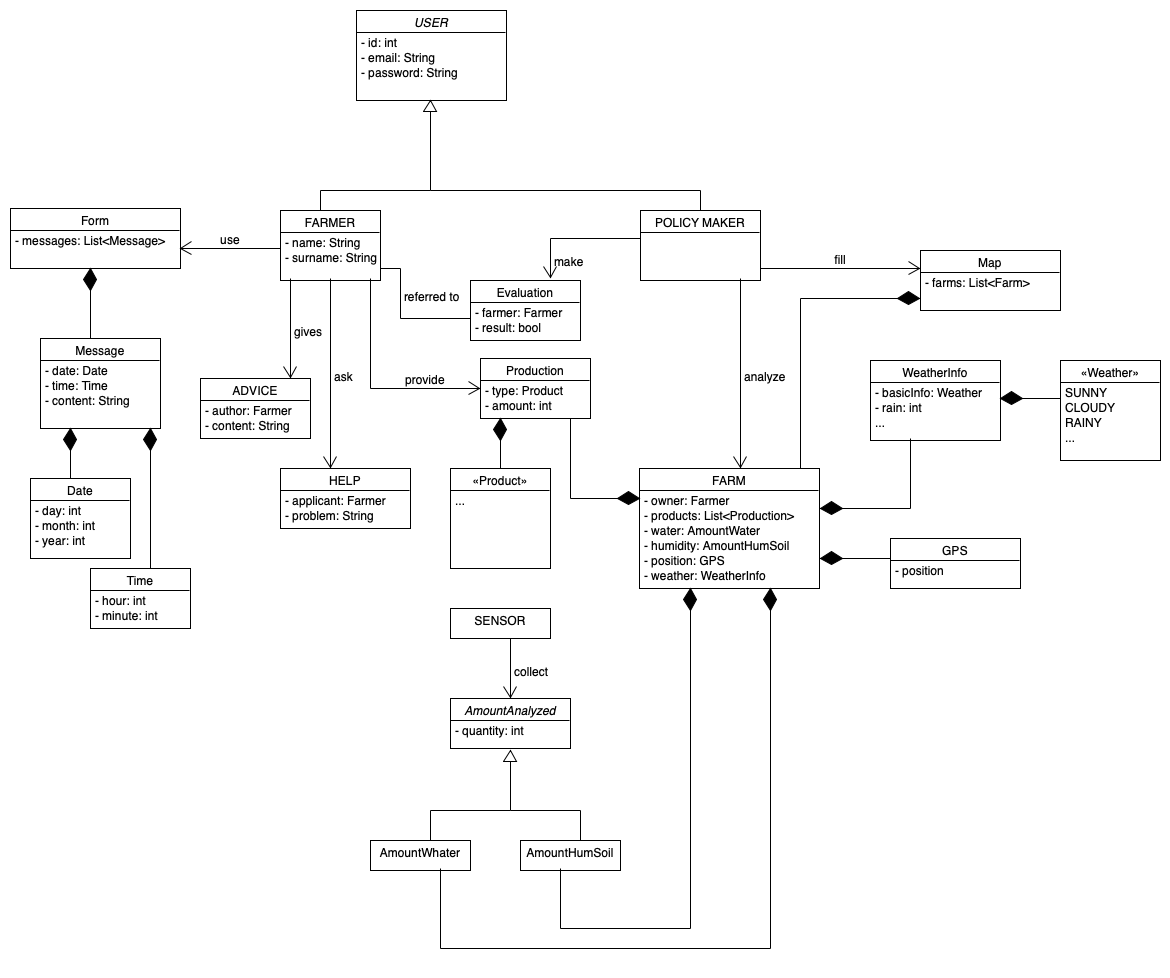
\includegraphics[width=1\textwidth]{images/UMLSW2_1.png}
    \caption{UML diagram.}
    \label{fig:dataaugmentation}
    \end{center}
\end{figure}
\subsection{State Diagram}
\subsection{Product Functions}
- insertion of data of production
- identify how farmers are performing
- farmers visualize relevant data 
- insertion of thing (request, suggestion, answer) in the forum
- interaction between farmers

\subsubsection{Scenario}

\end{document}
